\documentclass[10pt,a4paper,headinclude=true]{report}
\usepackage[latin1]{inputenc}
\usepackage[a4paper]{geometry}
\usepackage{amsmath}
\usepackage{amsfonts}
\usepackage{amssymb}
\usepackage{graphicx}
\usepackage{hyperref}
\usepackage{pdflscape} % dlia landscape orientation 
\hypersetup{colorlinks,citecolor=black,filecolor=black,linkcolor=black,urlcolor=black}
\usepackage{float}
\usepackage{setspace}

\renewcommand{\familydefault}{\sfdefault}

\begin{document}
\onehalfspacing
\title{Industrial Year placement report}
\author{Edgar Ivanov\\ edi@aber.ac.uk \\ \\ IY ICT \& Media Technician}
\date{\today}
\maketitle

\tableofcontents

\chapter{Organization}
Assume we know nothing \& take a funnel approach. Start broad i.e. brief history \&
size of university, how it is distributed, no. of departments, IS structure, your
team within IS, your place within the team

My industrial year employment took place at Aberystwyth University, in Information Services department. Aberystwyth University is an institution of higher education with research departments, which provides undergraduate and postgraduate education. AU is located in small Aberystwyth town, on the west coast of Wales, with average population of 15 thousand people. University was founded in 1872 and changed its name since then a few times. There are 17 academic departments and 27 service departments.

\section{Information Services}
I will describe how the IS looks like inside, mainly I will focus on the technical groups, but I will give a short overview of the other groups as well. On figure~\ref{fig:i-s-hierarchy-tree-march-2012} you can see IS hierarchy tree.

\begin{figure}[H]
\centering
\centerline{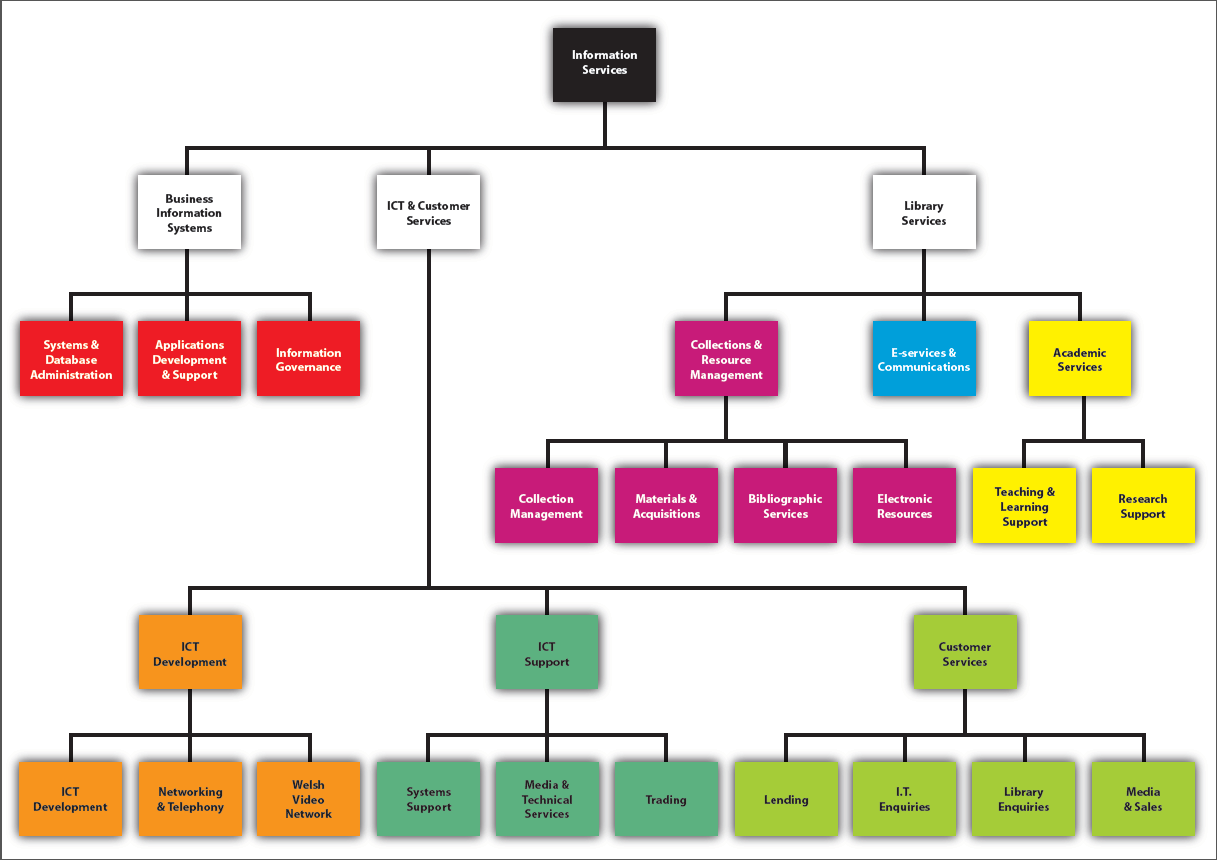
\includegraphics[scale=0.55]{./i-s-hierarchy-tree-march-2012}}
\caption{IS hierarchy tree}
\label{fig:i-s-hierarchy-tree-march-2012}
\end{figure}

\section{ICT Support}
\subsection{Media \& Technical Services}
The group that I am based in falls under IS -\textgreater ICT \& Customer Services -\textgreater ICT Support and is called "Media \& Technical Services". It is defined as a group responsible for the software and hardware upgrades and repairs a wide variety of ICT equipment types. It also provides multimedia services and supports ICT equipment within teaching spaces. This means that all computer relevant hardware repairs are done within this group, it includes internal repairs (the equipment owned by university ) as well as repairs for external customers (staff, students, members of publicity). The members of this group also provide technical support to lecturers who are teaching and experience any issues with teaching equipment.
\subsection{Systems Support}
This group is responsible for all the aspects of PSV workstations, including software licensing, purchasing, management and implementation for Information Services and many departmental products. It makes backups for most of the University's systems and maintains two main server rooms, one in Penglais and one in Gogerddan. It also provides second/third line software support for the help-desk/workshop.
\subsection{Trading}
Offers a wide range of computers, laptops, media equipment and peripherals for sale to University Departments, individuals and external customers. Prices are generally competitive and are often at specially negotiated educational terms and/or with extended warranties for the members of the University,
\section{ICT Development}
Designs and implements systems and services for IS, other University departments, and external bodies. Also develops, implements, trains and supports IS users on bespoke software and ensures existing systems are efficient and cost effective. This includes Network and Telephone service design promoting standardization and centralization and managing improvements and information security incidents.
\section{Customer Services}
Provides Lending, ICT enquiries, Media \& Sales and Library Enquiry services for staff, students and visitors. Monitors the responsiveness and effectiveness of front-line services, ensures services best meet users' needs and promotes awareness of IS enquiry and front-line services. It also manages services and staffing for Freshers' Weekends and students' induction programmes.

\subsection{I.T Enquiries}
I will give more details on I.T Enquiries group, where other IY's are based, since I work a few hours a week in this group as well as working for the Media and Technical services.

The first point of contact for face-to-face and online IT enquiries for all Information Services users. Troubleshoots any problems users experience with accessing or using Information Services services and resolves them or refers them as appropriate. Also supports the Public printing service, facilitates access to Information Services services such as email accounts, Aber cards, computing network, and printing and represents our users within IS e.g. presenting user feedback at meetings or user testing new services. I did two shifts a week on Service Point 2, helping customers with technical enquires and directing .

\section{BIS and Library Services}
There are also two other main groups called "Business Information Systems" and "Library Services". People in BIS are  responsible for development and support of the systems and processes required to maintain Admissions, Student Records, Finance, HR, Payroll and other associated business functions of the University. Library Services looks after all education materials: books, journals, articles as well as after education software systems like blackboard.


\section{People that I worked with}

\chapter{Technical environment}
When I just started my placement I was frustrated with amount of different software used in IS and how information was spread across all these systems. At the beginning I was introduced to Interzone, Sunrise, Astra, Recall, SharePoint, Aber FAQs, Outlook, Voyager. All used to store different information.

\section{Criticism}One of the issues I found that if I wanted to find some procedures I would need to check Sharepoint as well as Aber FAQs, since I could find what I need on any of this systems. Information about data projectors in teaching rooms is kept on SharePoint in simple Excel spreadsheet, which can be altered by anyone. Computer room layout with computer serial numbers kept on one of the employees M drive and is accessible through the web. So if Clares account will be locked for some reason, non of the workshop members will be able to access that data. Good example is PSR2 maintenance application which was clearly written by Clare for herself to make her job easier. On figure ~\ref{fig:main_PSR2_page} you can see main PSR2 page, which contains some teaching rooms list that workshop technicians looks after.

\begin{figure}[H]
\centering
\centerline{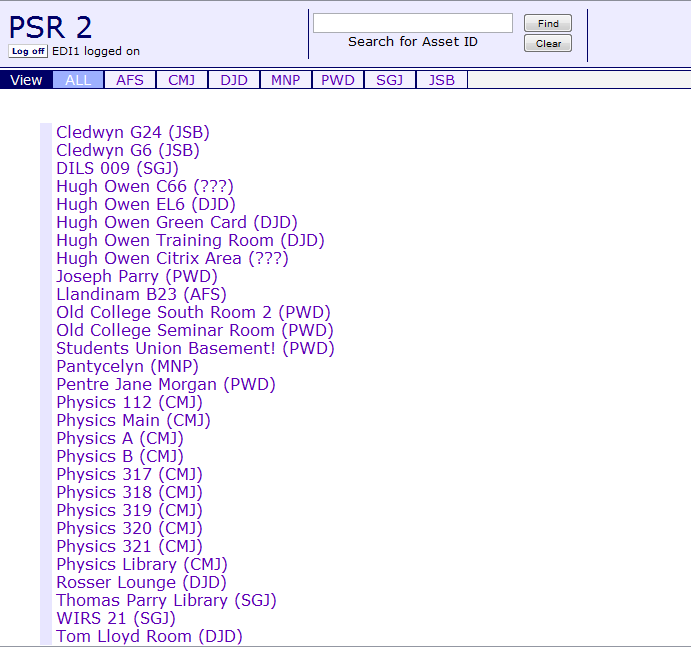
\includegraphics[scale=0.3]{./PSR2}}
\caption{Main PSR2 Page}
\label{fig:main_PSR2_page}
\end{figure}

Figure~\ref{fig:PSR2_SU_Room_layout} shows you Students Union computer room layout with computer names and serial numbers. Room comment holds code to unlock monitors from security straps. It also contains information when each computer was last time checked. So it contains quite 

\begin{figure}[H]
\begin{center}
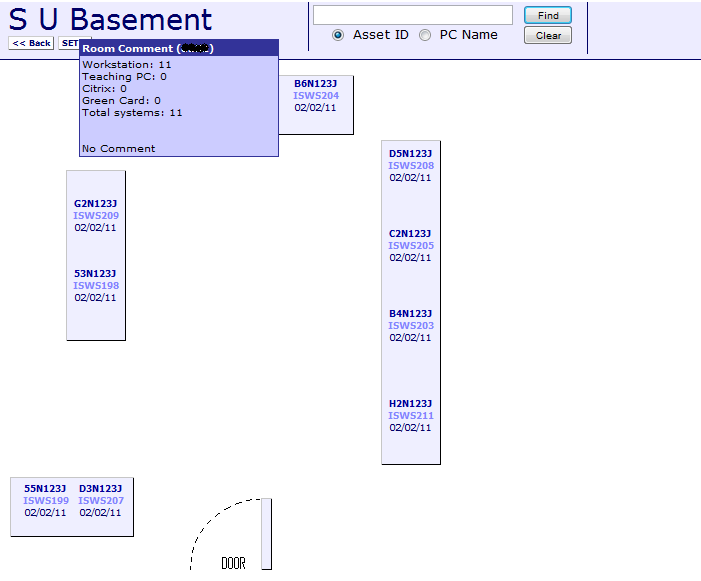
\includegraphics[scale=0.5]{./PSR2_SU_Room_layout}
\caption{PSR2 Students Union Computer Room Layout}
\label{fig:PSR2_SU_Room_layout}
\end{center}
\end{figure}


\section{Interzone}
Interzone is a web based application that is used to manage records of network equipment in Aberystwyth University. On the main page you can see blank boxes in which you enter the information and search for record that contains specified information in it. You can search by IP address, MAC address, Owner's login, computer name etc. On the figure ~\ref{fig:main_interzone_page} you can see main Interzone page.

\begin{figure}[H]
\centering
\centerline{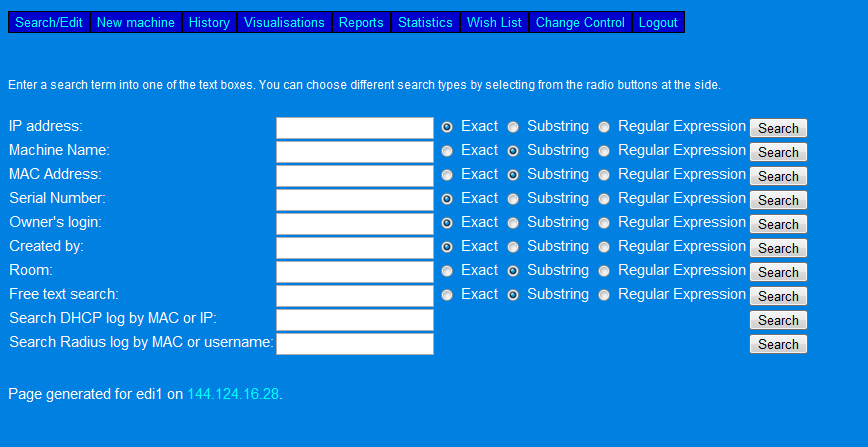
\includegraphics[scale=0.5]{./main_interzone_page}}
\caption{Main Interzone Page}
\label{fig:main_interzone_page}
\end{figure}

On figure ~\ref{fig:machine_record} you can see Interzone record for my computer.

\begin{figure}[H]
\centering
\centerline{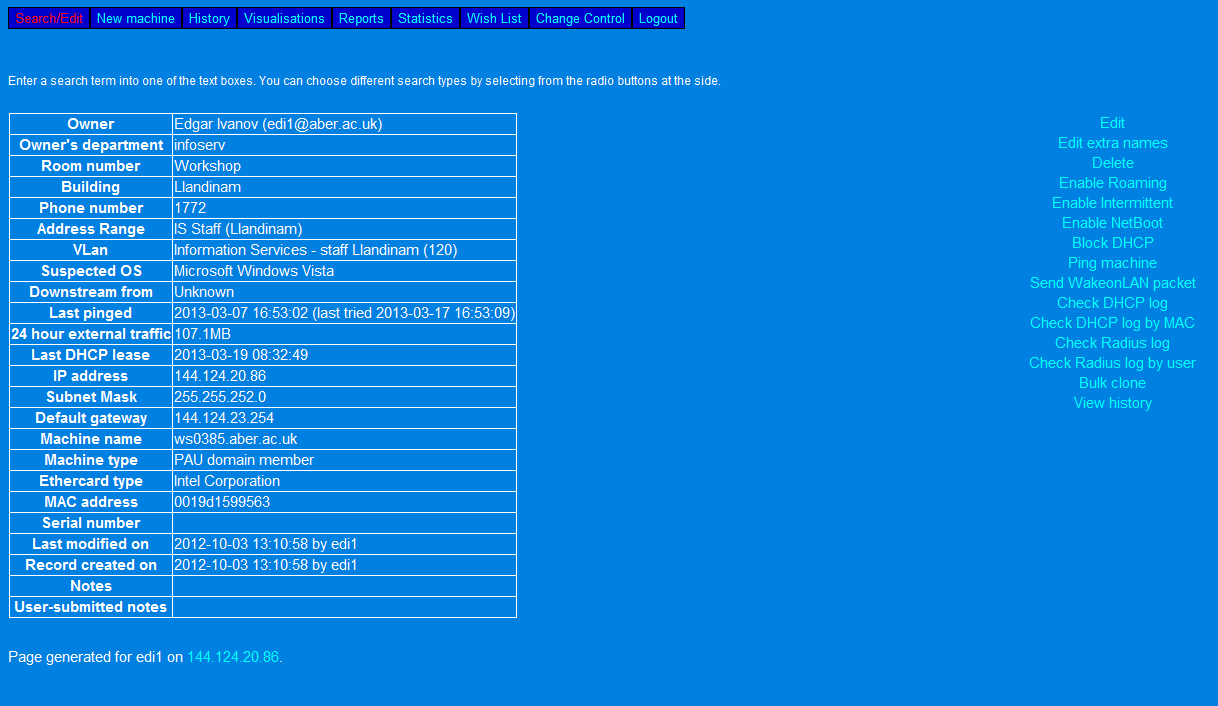
\includegraphics[scale=0.5]{./machine_record}}
\caption{Machine record}
\label{fig:machine_record}
\end{figure}

It contains various information about the owner, owners department, telephone number (if there is one), VLAN, IP and MAC addresses, you can also see who created this record and when it was last modified.

\begin{figure}[H]
\centering
\centerline{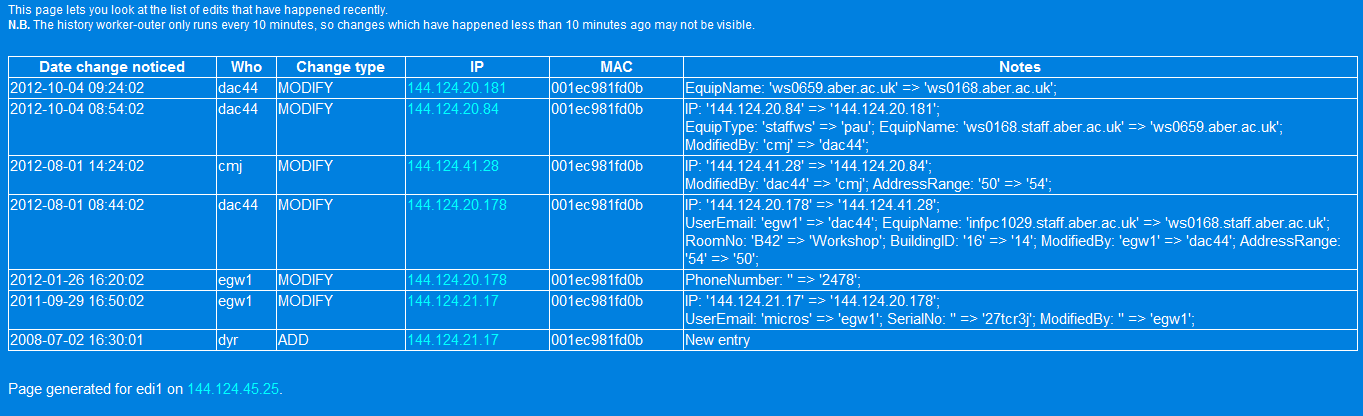
\includegraphics[scale=0.5]{./modification_history}}
\caption{Machine record}
\label{fig:modification_history}
\end{figure}


\chapter{What I did}
Describe your 'routine' weekly duties. Spend a bit more time on areas where you have
responsibility or have put in effort e.g. summer builds, FAQS, summer course
registrations, any exploratory projects or mini-projects you may have been given to
name a few

\chapter{Critical evaluation}

\end{document}
